\chapter{Resultados Experimentais}\label{result}

Este capítulo apresenta os resultados experimentais obtidos na indução do modelo \textit{Adaboost} sobre 30\% da base de conhecimento.

\subsection{Métricas utilizadas}

Avaliar o desempenho de um modelo é um dos estágios principais deste estudo, a avaliação se baseia nas predições que são produzidas pelo modelo induzido. 

Na comparação dos resultados experimentais serão utilizadas sete métricas de avaliações sobre modelo supervisionado \textit{AdaBoost}, que são:

\textbf{Matriz de confuzão} - A matriz de confusão de uma hipótese H oferece uma medida efetiva do modelo de classificação, ao mostrar o número de classificações corretas versus as classificações preditas para cada classe, sobre um conjunto de exemplos verdadeiros como descrito na Tabela ~\ref{tab:matrix_confusion}.

\begin{table}[H]
\centering
\caption{Matriz de confusão}
\begin{tabular}{rc|c|c|}
\cline{3-4}
\multicolumn{2}{c|}{\multirow{2}{*}{}} & \multicolumn{2}{c|}{Valor verdadeiro} \\ \cline{3-4} 
\multicolumn{2}{c|}{} & positivos & negativos \\ \hline
\multicolumn{1}{|c|}{\multirow{2}{*}{Valor previsto}} & positivos & VP & FP \\ \cline{2-4} 
\multicolumn{1}{|c|}{} & negativos & FN & VN \\ \hline
\end{tabular}
\label{tab:matrix_confusion}
\end{table}


\textbf{Acurácia} - porcentagem de amostras positivas e negativas classificadas corretamente sobre a soma de amostras positivas e negativas dada pela fórmula da equação ~\ref{eq:acuracia}:
\begin{equation} \label{eq:acuracia}
 acuracia = \frac{TP+TN}{VP+VN+FP+FN}
\end{equation}

\textbf{\textit{Recall}} - ou sensitividade é a porcentagem de amostras positivas classificadas corretamente sobre o total de amostras positivas dada pela fórmula da equação ~\ref{eq:recall}:
\begin{equation} \label{eq:recall}
  recall = \frac{TP}{TP+FN} = \frac{TP}{\textit{Positive}}
\end{equation}

\textbf{\textit{Precision}} - ou precisão é a porcentagem de amostras positivas classificadas corretamente sobre o total de amostras classificadas como positivas dada pela fórmula da equação ~\ref{eq:precision}:
\begin{equation} \label{eq:precision}
    precision = \frac{TP}{TP+FP}
\end{equation}

\textbf{\textit{Specificity}} - ou especificidade é a porcentagem de amostras negativas identificadas corretamente sobre o total de amostras negativas dada pela fórmula da equação ~\ref{eq:specificity}:
\begin{equation} \label{eq:specificity}
    specificity = \frac{TN}{TN+FP}=\frac{TN}{\textit{Negative}}
\end{equation}

\textbf{\textit{F-Score}} - ou \textit{F-Measure} é uma média ponderada de precisão e sensitividade dada pela fórmula da equação ~\ref{eq:fscore}:
\begin{equation} \label{eq:fscore}
    fscore=\frac{2*(\textit{Precision}*\textit{Recall})}{\textit{Precision}+\textit{Recall}}
\end{equation}

\textbf{Curva ROC} - a Curva ROC é um gráfico da porcentagem de amostras corretamente classificadas como positivas dentre todas as positivas reais versus a porcentagem de amostras erroneamente classificadas como positivas dentre todas as negativas reais ou um \textit{trade-off} entre TPR e FPR, dadas pelas fórmulas da equações  

\begin{equation} \label{eq:tpr}
    TPR=\frac{TP}{TP+FN}
\end{equation}

\begin{equation} \label{eq:fpr}
    FPR=\frac{FP}{FP+TN}
\end{equation}

Obviamente, um modelo de classificação ideal teria TPR = 1 e FPR = 0 (taxa de acerto = 1 e taxa de erro = 0).

\subsection{Analise de precisão}

\begin{table}[]
\centering
\begin{tabular}{c|c|c|c|c|c|}
\cline{2-6}
 & \multicolumn{5}{c|}{\textbf{Resultado da avaliação}} \\ \hline
\multicolumn{1}{|c|}{\textbf{Classes}} & \textbf{ROC} & \textbf{Acurácia} & \textit{\textbf{F-Score}} & \textit{\textbf{Precision}} & \textit{\textbf{Recall}} \\ \hline
\multicolumn{1}{|c|}{\textbf{0.00}} & 0.498 & 0.828 & 0.096 & 0.845 & 0.828 \\ \hline
\multicolumn{1}{|c|}{\textbf{0.50}} & 0.552 & 0.640 & 0.349 & 0.653 & 0.640 \\ \hline
\multicolumn{1}{|c|}{\textbf{1.00}} & 0.499 & 0.509 & 0.422 & 0.506 & 0.509 \\ \hline
\multicolumn{1}{|c|}{\textbf{1.50}} & 0.54 & 0.579 & 0.222 & 0.755 & 0.759 \\ \hline
\multicolumn{1}{|c|}{\textbf{2.00}} & 0.541 & 0.915 & 0.140 & 0.899 & 0.915 \\ \hline
\end{tabular}
\caption{My caption}
\label{my-label}
\end{table}

\begin{figure}[H]
\begin{center}
    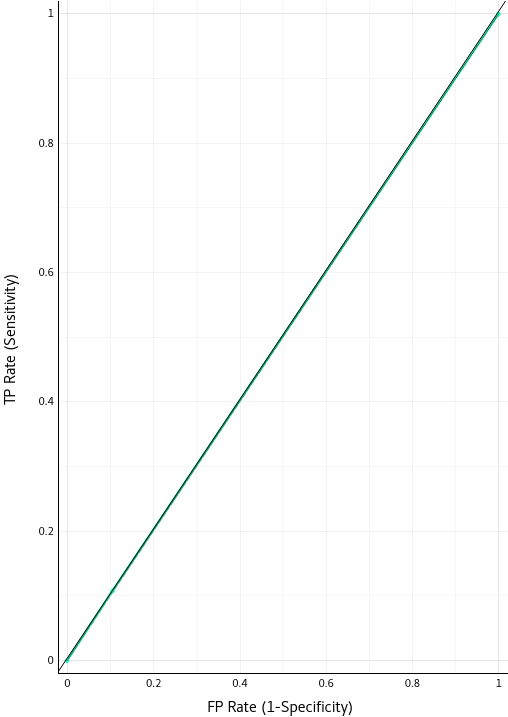
\includegraphics{figuras/roc_0-0.png}
\end{center}
\caption{}
\label{fig:class_0.00}
\end{figure}

\begin{figure}[H]
\begin{center}
    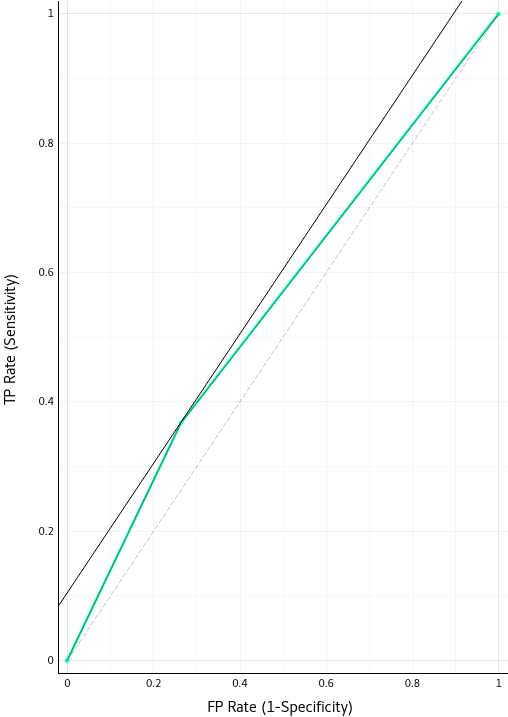
\includegraphics{figuras/roc_0-5.png}
\end{center}
\caption{}
\label{fig:class_0.50}
\end{figure}

\begin{figure}[H]
\begin{center}
    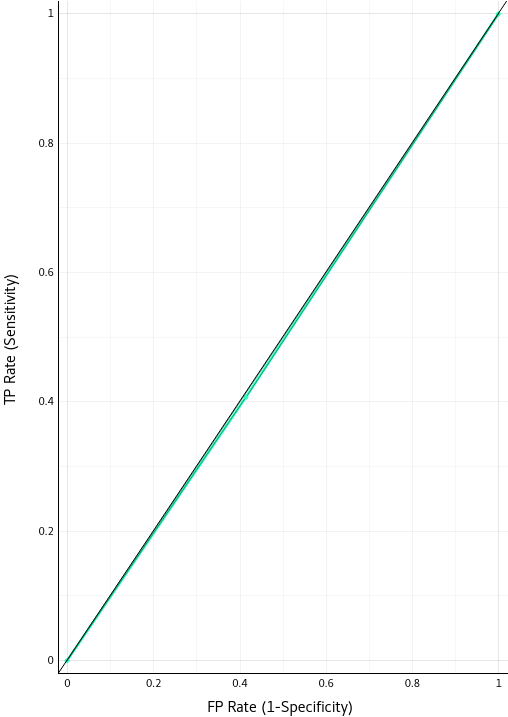
\includegraphics{figuras/roc_1-0.png}
\end{center}
\caption{}
\label{fig:class_1.00}
\end{figure}

\begin{figure}[H]
\begin{center}
    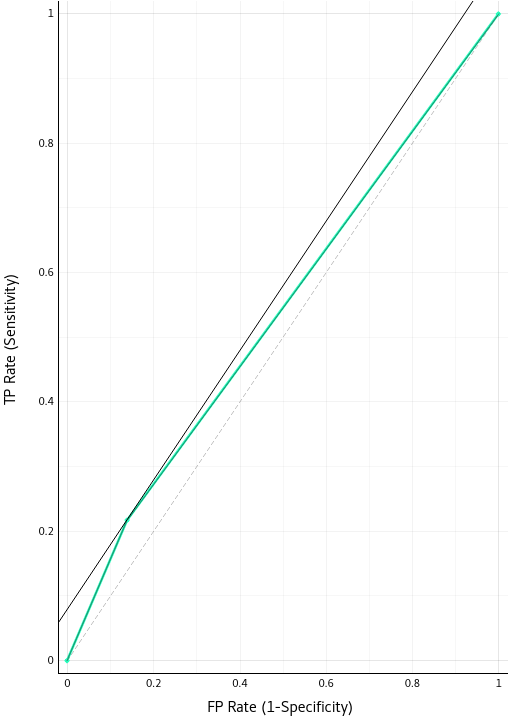
\includegraphics{figuras/roc_1-5.png}
\end{center}
\caption{}
\label{fig:class_1.50}
\end{figure}

\begin{figure}[H]
\begin{center}
    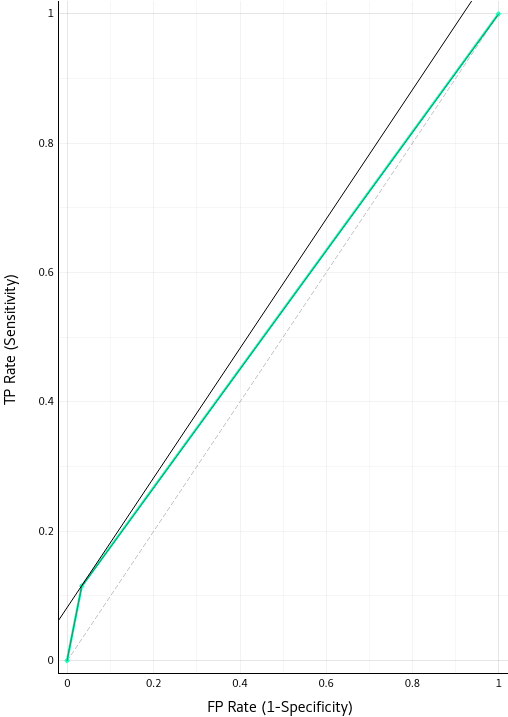
\includegraphics{figuras/roc_2-0.png}
\end{center}
\caption{}
\label{fig:class_2.00}
\end{figure}

\begin{table}[H]
\centering
\caption{My caption}
\label{my-label}
\begin{tabular}{cc|c|c|c|c|c|c|}
\cline{3-8}
 &  & \multicolumn{6}{c|}{Predição} \\ \cline{3-8} 
 &  & 0.00 & .050 & 1.00 & 1.50 & 2.00 & $\sum_{}$  \\ \hline
\multicolumn{1}{|c|}{} & 0.00 & \cellcolor[HTML]{C0C0C0}4 & 18 & 13 & 2 & 0 & \textbf{37} \\ \cline{2-8} 
\multicolumn{1}{|c|}{} & 0.50 & 13 & \cellcolor[HTML]{C0C0C0}42 & 44 & 14 & 1 & \textbf{114} \\ \cline{2-8} 
\multicolumn{1}{|c|}{} & 1.00 & 18 & 51 & \cellcolor[HTML]{C0C0C0}78 & 32 & 11 & \textbf{190} \\ \cline{2-8} 
\multicolumn{1}{|c|}{} & 1.50 & 7 & 14 & 31 & \cellcolor[HTML]{C0C0C0}15 & 2 & \textbf{69} \\ \cline{2-8} 
\multicolumn{1}{|c|}{} & 2.0 & 4 & 2 & 14 & 3 & \cellcolor[HTML]{C0C0C0}3 & \textbf{26} \\ \cline{2-8} 
\multicolumn{1}{|c|}{\multirow{-6}{*}{\rot{Atual}}} & $\sum_{}$ & \textbf{46} & \textbf{127} & \textbf{180} & \textbf{66} & \textbf{17} & \textbf{436} \\ \hline
\end{tabular}
\end{table}

Os primeiros experimentos realizados na predição, ilustrado no Gráfico abaixo, demonstraram uma taxa de 30\% de acerto na predição da primeira competência exigida em um texto de redação, de uma amostra de 100 redações. 

A análise gráfica do resultado experimental demonstra que a predição do modelo está em uma faixa especifica de 0.5 a 1.5, ou seja, a indução do modelo deve ser repetida até o mesmo se tornar genérico.

\pgfplotstableread[col sep=semicolon]{data/adaboost_competence_1.dat}\data
\begin{figure}[H]
\begin{center}

\begin{tikzpicture}
    \begin{axis}[
        title=Demonstrar domínio da norma padrão da língua escrita. (1ªCompetência ),
        width=\textwidth,
        ymin=0,
        ytick={0,0.5,1.0,1.5,2.0},
        ylabel=Pontuação,
        xtick=data,
        xticklabel style={rotate=90,anchor=east},
        xticklabels from table={\data}{title},
        legend style={ legend columns=-1},
        enlarge x limits=0.01,
        ]
        \addplot table[x=id, y=comp1] {\data};
        \addplot table[x=id, y=adaboost] {\data};
        \legend{Profissional,AdaBoost}
    \end{axis}
\end{tikzpicture}
\end{center}
\end{figure}

